\documentclass{beamer}
\usepackage[utf8]{inputenc}

\usetheme{Madrid}
\usecolortheme{default}
\usepackage{amsmath,amssymb,amsfonts,amsthm}
\usepackage{txfonts}
\usepackage{tkz-euclide}
\usepackage{listings}
\usepackage{adjustbox}
\usepackage{array}
\usepackage{tabularx}
\usepackage{gvv}
\usepackage{lmodern}
\usepackage{circuitikz}
\usepackage{tikz}
\usepackage{graphicx}

\setbeamertemplate{page number in head/foot}[totalframenumber]

\usepackage{tcolorbox}
\tcbuselibrary{minted,breakable,xparse,skins}

\definecolor{bg}{gray}{0.95}
\DeclareTCBListing{mintedbox}{O{}m!O{}}{%
breakable=true,
listing engine=minted,
listing only,
minted language=#2,
minted style=default,
minted options={%
linenos,
gobble=0,
breaklines=true,
breakafter=,,
fontsize=\small,
numbersep=8pt,
#1},
boxsep=0pt,
left skip=0pt,
right skip=0pt,
left=25pt,
right=0pt,
top=3pt,
bottom=3pt,
arc=5pt,
leftrule=0pt,
rightrule=0pt,
bottomrule=2pt,
toprule=2pt,
colback=bg,
colframe=orange!70,
enhanced,
overlay={%
\begin{tcbclipinterior}
\fill[orange!20!white] (frame.south west) rectangle ([xshift=20pt]frame.north west);
\end{tcbclipinterior}},
#3,
}
\lstset{
language=C,
basicstyle=\ttfamily\small,
keywordstyle=\color{blue},
stringstyle=\color{orange},
commentstyle=\color{green!60!black},
numbers=left,
numberstyle=\tiny\color{gray},
breaklines=true,
showstringspaces=false,
}



\title 
{1.5.30}
\date{August 28, 2025}

\author
{EE25BTECH11043 - Nishid Khandagre}

\begin{document}

\frame{\titlepage}
\begin{frame}{Question}
If the coordinates of one end of a diameter of a circle are $\myvec{2\\3}$ and the coordinates of its centre are $\myvec{-2\\5}$ , then the coordinates of the other end of the diameter are?
\end{frame}


\begin{frame}{Theoretical Solution}

Let the coordinates of the known end of the diameter be vector $\vec{B}$. \
Let the coordinates of the center of the circle be vector $\vec{P}$. \
Let the coordinates of the other end of the diameter be vector $\vec{A}$ (the required vector).

\end{frame}
\begin{frame}
Given:
\begin{align}
\vec{B} &= \myvec{2 \\ 3} \\
\vec{P} &= \myvec{-2 \\ 5}
\end{align}

\end{frame}

\begin{frame}{Equation}

The center of a circle is the midpoint of its diameter. For a circle with center $\vec{P}$ and ends of diameters represented by vectors $\vec{A}$ and $\vec{B}$, the relationship is:
\begin{align}
\vec{P}=\frac{\vec{A}+\vec{B}}{2}
\end{align}

\end{frame}

\begin{frame}{Theoretical Solution}

To find vector $\vec{A}$, we use the midpoint formula. We know that $\vec{P}$ divides diameter $\vec{AB}$ in ratio 1:1.

Substituting the given values into the equation:
\begin{align}
\vec{P} &= \frac{\vec{A} + \myvec{2 \\ 3}}{2} \\
2 \cdot \myvec{-2 \\ 5} &= \vec{A} + \myvec{2 \\ 3} \\
\myvec{-4 \\ 10} &= \vec{A} + \myvec{2 \\ 3}
\end{align}

\end{frame}

\begin{frame}{Theoretical Solution}
Rearranging the terms to solve for $\vec{A}$:
\begin{align}
\vec{A} &= \myvec{-4 \\ 10} - \myvec{2 \\ 3} \\
\vec{A} &= \myvec{-4 - 2 \\ 10 - 3}
\end{align}
Hence, the coordinates of the other end of the diameter are:
\begin{align}
\vec{A} = \myvec{-6 \\ 7}
\end{align}

\end{frame}

\begin{frame}[fragile]
\frametitle{C Code }


\begin{lstlisting}
#include <stdio.h>

// Function to calculate the coordinates of the other end of the diameter
void formula(double x1, double y1, double xc, double yc, double *x2, double *y2) {
    *x2 = 2 * xc - x1;
    *y2 = 2 * yc - y1;
}
\end{lstlisting}
\end{frame}

\begin{frame}[fragile]
\frametitle{C Code }
\begin{lstlisting}
int main() {
    double x1 = 2;
    double y1 = 3;
    double xc = -2;
    double yc = 5;
    double x2, y2;

    formula(x1, y1, xc, yc, &x2, &y2);

    return 0;
}

\end{lstlisting}
\end{frame}

\begin{frame}[fragile]
\frametitle{Python Code through shared output }

\begin{lstlisting}
import ctypes
import numpy as np
import matplotlib.pyplot as plt

# Load the shared library
lib_diameter = ctypes.CDLL("./code.so")

# Define the argument types and return type for the C function
lib_diameter.findOtherEndOfDiameter.argtypes = [
    ctypes.c_double,  # x1
    ctypes.c_double,  # y1
    ctypes.c_double,  # xc
    ctypes.c_double,  # yc
    ctypes.POINTER(ctypes.c_double), # x2
    ctypes.POINTER(ctypes.c_double)  # y2
    \end{lstlisting}
    \end{frame}
    \begin{frame}[fragile]
\frametitle{Python Code through shared output }

\begin{lstlisting}
]
lib_diameter.findOtherEndOfDiameter.restype = None

# Given coordinates
x1_given, y1_given = 2.0, 3.0  # One end of the diameter
xc_given, yc_given = -2.0, 5.0  # Center of the circle

# Create ctypes doubles to hold the results
x2_result = ctypes.c_double()
y2_result = ctypes.c_double()

# Call the C function to find the other end of the diameter
lib_diameter.findOtherEndOfDiameter(
    x1_given, y1_given,
    xc_given, yc_given,
    ctypes.byref(x2_result),
    ctypes.byref(y2_result)
)
\end{lstlisting}
\end{frame}
\begin{frame}[fragile]
\frametitle{Python Code through shared output  }

\begin{lstlisting}

x2_found = x2_result.value
y2_found = y2_result.value

print(f"The coordinates of the other end of the diameter are ({x2_found:.2f}, {y2_found:.2f})")

# Calculate the radius for plotting the circle
radius = np.sqrt((x1_given - xc_given)**2 + (y1_given - yc_given)**2)

# Generate points for the circle
theta = np.linspace(0, 2 * np.pi, 200)
circle_x = xc_given + radius * np.cos(theta)
circle_y = yc_given + radius * np.sin(theta)

\end{lstlisting}
\end{frame}
\begin{frame}[fragile]
\frametitle{Python Code through shared output }

\begin{lstlisting}
# Plotting
plt.figure(figsize=(8, 8))

# Plot the circle
plt.plot(circle_x, circle_y, 'b-', label='Circle')

# Plot the given diameter end
plt.scatter(x1_given, y1_given, color='red', s=100, zorder=5)
plt.annotate(f'({x1_given},{y1_given})', (x1_given, y1_given), textcoords="offset points", xytext=(5,5), ha='left')

\end{lstlisting}
\end{frame}
\begin{frame}[fragile]
\frametitle{Python Code through shared output  }

\begin{lstlisting}
# Plot the center
plt.scatter(xc_given, yc_given, color='green', s=100, zorder=5)
plt.annotate(f'({xc_given},{yc_given})', (xc_given, yc_given), textcoords="offset points", xytext=(5,5), ha='left')

# Plot the calculated other end of the diameter
plt.scatter(x2_found, y2_found, color='purple', s=100, zorder=5)
plt.annotate(f'({x2_found:.2f},{y2_found:.2f})', (x2_found, y2_found), textcoords="offset points", xytext=(5,5), ha='left')

\end{lstlisting}
\end{frame}
\begin{frame}[fragile]
\frametitle{Python Code through shared output }

\begin{lstlisting}

plt.plot([x1_given, x2_found], [y1_given, y2_found], 'r--', label='Diameter')

plt.gca().set_aspect('equal', adjustable='box')
plt.xlabel('X-axis')
plt.ylabel('Y-axis')
plt.title('Circle and its Diameter')
plt.grid(True)
plt.legend()
plt.show()



\end{lstlisting}

\end{frame}
\begin{frame}[fragile]
\frametitle{Python Code : Direct}

\begin{lstlisting}
import sys
import numpy as np
import numpy.linalg as LA
import matplotlib.pyplot as plt


def line_gen_num(A, B, num_points):
   
    A = A.flatten()
    B = B.flatten()
    t = np.linspace(0, 1, num_points)
    points = np.outer(A, (1-t)) + np.outer(B, t)
    return points
\end{lstlisting}
\end{frame}

\begin{frame}[fragile]
\frametitle{Python Code : Direct }

\begin{lstlisting}

def circ_gen(center, radius, num_points=100):
  
    center = center.flatten()
    theta = np.linspace(0, 2*np.pi, num_points)
    x = center[0] + radius * np.cos(theta)
    y = center[1] + radius * np.sin(theta)
    return np.array([x, y])

# Given coordinates
B = np.array([2, 3]).reshape(-1, 1)  
P = np.array([-2, 5]).reshape(-1, 1) 
\end{lstlisting}
\end{frame}

\begin{frame}[fragile]
\frametitle{Python Code : Direct }

\begin{lstlisting}

# Function to calculate the other end of the diameter
def func_other_end(center, one_end):
    return 2 * center - one_end

# Function to calculate the radius
def func_radius(center, point_on_circumference):
    return LA.norm(center - point_on_circumference)

# Calculate the other end of the diameter (A)
A = func_other_end(P, B).reshape(-1, 1)

# Calculate the radius of the circle
radius = func_radius(P, B)
\end{lstlisting}
\end{frame}

\begin{frame}[fragile]
\frametitle{Python Code : Direct }

\begin{lstlisting}

print(f"The coordinates of the other end of the diameter are ({A[0,0]}, {A[1,0]})")

# Generate points for the diameter line
x_AB = line_gen_num(A, B, 20)

# Generate points for the circle
x_circ = circ_gen(P, radius)

# Plotting
plt.plot(x_circ[0,:], x_circ[1,:], "red", label="Circle")
plt.plot(x_AB[0,:], x_AB[1,:], "g--", label="Diameter")

# Plot the points
tri_coords = np.block([[A, B, P]])
plt.scatter(tri_coords[0,:], tri_coords[1,:], s=50, zorder=5) # s for size, zorder to ensure visibility
\end{lstlisting}
\end{frame}
\begin{frame}[fragile]
\frametitle{Python Code : Direct }

\begin{lstlisting}

# Add labels to the points
vert_labels = [f'A({A[0,0]:.0f},{A[1,0]:.0f})', f'B({B[0,0]:.0f},{B[1,0]:.0f})', f'P({P[0,0]:.0f},{P[1,0]:.0f}) (Center)']
for i , txt in enumerate(vert_labels):
    plt.annotate(txt, (tri_coords[0,i], tri_coords[1,i]), textcoords="offset points", xytext=(5,5), ha='left')

plt.xlabel('$x$')
plt.ylabel('$y$')
plt.legend(loc='best')
plt.grid()
plt.title("Diameter of a Circle")
plt.axis('equal') # Important to make the circle appear circular
plt.savefig("fig1.png")
plt.show()

print("Figure saved as fig1.png")

\end{lstlisting}

\end{frame}

\begin{frame}{Plot by Python only}
\begin{figure}[H]
        \centering
        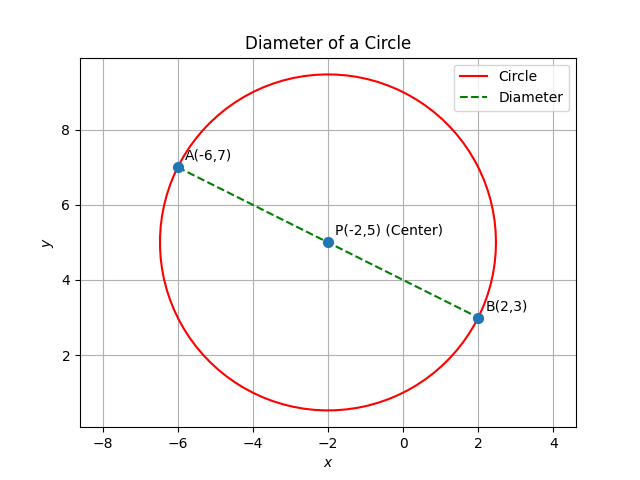
\includegraphics[width=0.7\columnwidth]{../figs/fig1.png}
        \caption{}
        \label{fig:1}
    \end{figure}
\end{frame}


\begin{frame}{Plot by Python using shared output from C}
\begin{figure}[H]
        \centering
        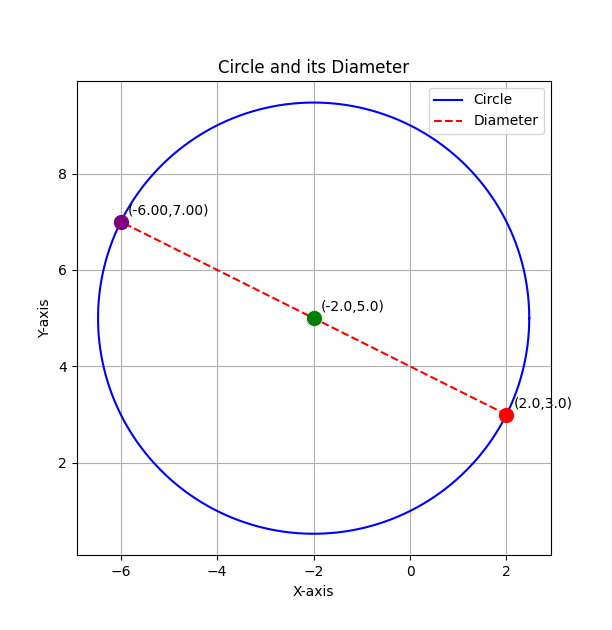
\includegraphics[width=0.7\columnwidth]{../figs/fig2.png}
        \caption{}
        \label{fig:2}
    \end{figure}
\end{frame}
 


\end{document}